\documentclass[a4paper]{article}
\usepackage{verbatim}
\usepackage{graphicx}

\title{Software Reengineering Project \\ Evolving \emph{ChEOPSJ}: from a prototype to a tool}
\author{Alejandro Merlo\\ Viktor Stojkovski\\ Rafael Ugaz}
\date{June, 2013}

\begin{document}
\maketitle

\section{Introduction}
For this re-engineering project, we have the task of improving the current implementation of the \emph{ChEOPSJ} system to support the storing and managing of changes with a more fine-grained level of detail. This means that the tool should be re-engineered so it can easily include support for local variables, full method signatures, and accesses of fields, local variables or parameters.

\section{First Contact}
In this section, we describe the initial steps that we took when we first encountered the system. The section is divided (as well as the whole report) in subsections representing a re-engineering pattern from \cite{demeyer02} that has been applied.

\subsection{Read all the code in one hour}
\label{sec:codeOneHour}
For this task we saw that the \emph{ChEOPSJ} system is split into ten projects, so we decided to divide them among the three members of our group. Each member read the code of their corresponding projects in around one hour and took notes. Then we explained our findings to each other in a meeting and merged the notes together to produce the report shown below. Because of the `time is scarce' principle, we payed more attention to the following items, as it is proposed in \cite{demeyer02}:
\begin{itemize}
\item Abstract classes and methods, that reveal design intentions.
\item Classes high in the hierarchy, which often define domain abstractions; their subclasses introduce variations on a theme.
\item Occurrences of the Singleton pattern that may represent information that is constant for the entire execution of a system.
\item Surprisingly large structures, which often specify important chunks of functionality.
\item Comments, that can reveal a lot about the design intentions behind a particular piece of code, yet may often be misleading.
\end{itemize}

The notes taken, separated by project and ordered alphabetically, are the following:

% cheopsj
\subsubsection{be.ac.ua.ansymo.cheopsj}
The project \emph{be.ac.ua.ansymo.cheopsj} only contains the feature.xml file with references to all the other plugins which groups them together as a whole as the \emph{ChEOPSJ} plugin for Eclipse. Most of the other plug-in projects contain an Activator class that controls the project's plug-in life cycle.

\subsubsection{be.ac.ua.ansymo.cheopsj.branding}
% branding
The project \emph{be.ac.ua.ansymo.cheopsj.branding} contains an about.html website and seems to be related to the plugin information displayed when browsing the plugin to install it in Eclipse.

\subsubsection{be.ac.ua.ansymo.cheopsj.changerecorders}
% changerecorders
The project \emph{be.ac.ua.ansymo.cheopsj.changerecorders} is the first with actual source code. It contains the datastructures used for storing the changes of each type of entity (e.g. class, method or variable).
The AbstractEntityRecorder is at the top of the hierarchy subclassed by all recorders in the package. The StatementRecorder is also abstract but subclassed only by LocalVariable and MethodInvocation recorders, it adds extra common methods to them. All recorders inherit the storeChange method which uses the the abstract methods createAndLinkFamixElement and createAndLinkChange methods, which are implemented differently by each recorder subclass. These two methods, like their names indicate, create and link the famix element object and the change object to the recorder object.

Some classes related to one of the improvements that we must reengineer (support changes of accesses of fields and local variables) are also found in this project but have been excluded from the build path (probably unfinished) so we should look into them later and could use them as a basis.

There are a few comments in the code. Some are meant for the programmer himself, reminding him of things he has to do and some of them are informative but also a bit redundant because the functionality can be easily understood from the (good) naming of the methods or variables.

The tests found check if the change recorders work correctly for additions and removals of the corresponding java element (project, package, class, etc)

% distiller	
\subsubsection{be.ac.ua.ansymo.cheopsj.distiller}
In \emph{be.ac.ua.ansymo.cheopsj.distiller} one of the main functionalities of \emph{ChEOPSJ} is implemented. The one of extracting the changes from an existing java project. This is done by connecting to a SVN repository and then \emph{distilling} the changes that happen in each revision by means of an external library ChangeDistiller from the Evolizer platform.

In the \emph{distiller.cd} package, the class ChangeDistillerProxy accesses the API of the ChangeDistiller library to extract the source code changes from two java files.

In \emph{distiller.popup.actions} the actions taken when the user selects "Distill Changes" and "Distill Additions" from the popup or context menu are implemented. 

Finally, \emph{distiller.svnconnection} takes care of connecting and extracting the revisions from the SVN repository. Here we also saw that the SVN url is hardcoded to a path in the machine of a programmer and this could cause problems so we should also look into this in the future.

There are no tests present in this project.

% logger	
\subsubsection{be.ac.ua.ansymo.cheopsj.logger}
The \emph{be.ac.ua.ansymo.cheopsj.logger} project takes care of the second main functionaility of \emph{ChEOPSJ} which is to \emph{log} new changes made to the workspace by the user. In the \emph{logger} package, there are some classes for the initialization of the plug-in on Eclipse. It is important to note that the Cheopsj class employs the singleton pattern which means it is constant during the entire execution of the system.

The \emph{logger.astdiffer} package contains the classes ASTComparator and DiffVisitor, the first class instantiates the second in order to obtain the differences of two input Abstract Syntax Trees (AST), which are instances of the eclipse internal class CompilationUnit. The objective of this classes seems to be to compare two states of a workspace or compilation unit and in this way identify (and log) the changes that the user has made.

In the \emph{logger.listeners} package, we find two classes that take care of the listening to change events and then logging them. From the comments we can infer that it records the fine grained changes made inside the Java editor. The ChangeRecorder class also applies the singleton pattern.

Lastly, the \emph{logger.util} package contains some helper classes for the whole workspace. Although the Constants class is currently not being used anywhere. 
The project also contains some tests that should look into further.

The project contains some tests that we should look into further.

% model	
\subsubsection{be.ac.ua.ansymo.cheopsj.model}
The project \emph{be.ac.ua.ansymo.cheopsj.model} contains the main change model, which is composed of type of changes as well as type of entities. It also contains a model manager class which seems to be used extensively across the whole system. The ModelManager applies the singleton pattern, which confirms its importance in the system. Among the tasks that the manager performs, are the storing of all the Famix entities in several hash maps as well as all the changes that have been made to them. It also adds a listener which is an instance of the class ModelManagerListener that responds whenever whenever a ModelManagerEvent is thrown, which happens when a change is added to the model.

The package \emph{model.changes} contains all the types of change possible, with the Change class at the top of the hierarchy and also implementing the IChange interface. One level below in the hierarchy are the AtomicChange and CompositeChange classes and in the lowest the more specific Add, Modify and Remove. Finally the Subject abstract class represents and contains the functionalities of the element affected by the changes.

The \emph{model.famix} package contains the classes that represent all the entities for which changes will be stored. The FamixObject abstract class is at the top of the hierarchy and is extended directly or indirectly by all the classes in the package. It also extends the Subject class from the \emph{model.changes} package explained earlier, which gives all famix objects the functionalities needed to store and manage it's changes. Once we go deeper in the hierarchy, the classes contain more specific methods for the corresponding type of entity they represent (e.g. class, attribute or method).

There are no tests present in this project.

% model.ui
\subsubsection{be.ac.ua.ansymo.cheopsj.model.ui}
The project \emph{be.ac.ua.ansymo.cheopsj.model.ui} contains the implementation of the user interface. It is divided in 3 packages. \emph{ui.handlers} contains several event handlers for different events. These events are specified in the plugin.xml file and seem to be thrown whenever the corresponding command is called (e.g. for opening the view and to save or load a state).

The \emph{ui.changeinspector} package seems to contain the classes relevant to the change inspector view. The class ChangeSorter implements the functionality to sort (in ascending or descending) the changes in this view. The other classes create the viewer and update the content on it. 

Similarly to the change inspector view, the \emph{ui.changegraph} package contains the implementation for the change graph view.

This project deals exclusively with the graphical interface and it should not be necessary to modify in order to add new features.

There are no tests present in this project.

% testtool
\subsubsection{be.ac.ua.ansymo.cheopsj.testtool}
The plugin implemented in \emph{be.ac.ua.ansymo.cheopsj.testtool} is used for finding tests relevant to a set of changes. This is another mentioned functionality of \emph{ChEOPSJ}, namely to provide the user the tests that depend on an entity (e.g. class or method) and that would have to be checked for correctness after that entity has been modified. From the comments we can see that the functionality of the main method findTests is to, first, find the method where the selected change is in and, second, find the tests that call that method, in other words the relevant tests.

There are no tests present in this project.

% update
\subsubsection{be.ac.ua.ansymo.cheopsj.update}
The project \emph{be.ac.ua.ansymo.cheopsj.update} contains information about the update site of the \emph{ChEOPSJ} plugin

% evolizer.changedistiller
\subsubsection{org.evolizer.changedistiller}
This project contains the external library for extracting source code changes from two java files used in the \emph{be.ac.ua.ansymo.cheopsj.distiller} project.

\subsubsection{Conclusion}
In conclusion, the naming conventions of the whole workspace seem appropriate and help understanding the code much faster. The separation of classes into projects and into packages also states the intention of each group of classes more clearly. The comments could be better, but then again because of the facts just mentioned, they are not always needed. Finally, only two projects (changerecorders and logger) contain tests, the logger is an important part of \emph{ChEOPSJ} because it implements on of its main functionalities i.e. logging new changes for a project. In the other hand, the distiller project takes care of the other main functionality of \emph{ChEOPSJ}, which is distilling changes from an existing project, but it does not contain tests. It is possible that we will need to implement tests for this project in the future. The model project seems also very relevant (specially the model manager) and does not have any tests either.

\subsection{Skim the Documentation}
We could not really apply this pattern because of the scarce documentation found for the project. The assignment website and the project's site provide information on the features the \emph{ChEOPSJ} plugin performs but not how it performs them. An image which we found useful to get a big picture of how the different subsystems are integrated can be seen in Figure \ref{fig:skim}

\begin{figure}[h]
\centering
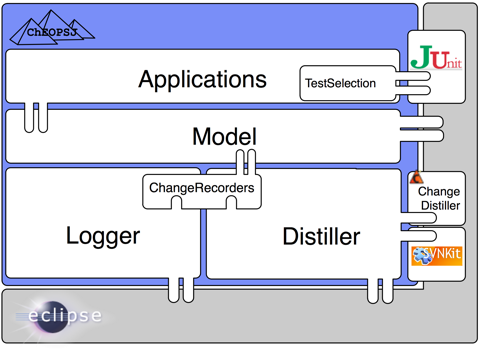
\includegraphics[width=0.8\textwidth]{Images/skim}
\caption{A big picture view of how the subsystems of \emph{ChEOPSJ} interact}
\label{fig:spec0}
\end{figure}

\subsection{Interview During Demo}
This pattern was also not fully applied because we did not perform an interview during a demo. We found a demo recorded as a video on the website of the project, and also saw some screenshots of it in action. Finally we tried the plugin ourselves doing a Mock Installation like it is explained in Section \ref{sec:mock}.

\subsection{Do a Mock Installation}
\label{sec:mock}
The first time we tried build the system in eclipse, we encountered some errors that prevented us doing it. A few plug-ins were missing, namely the SVN Team Provider and also the SWT library was not found in our Eclipse installation. After we solved this two problems all the errors disappeared and we were able to build the system. 

With the system running, we added a mock project to the workspace along with some packages and classes to see the functionality of the system. We noticed from the console that some exceptions were thrown while adding new elements in the java editor saying that the elements could not be found. It would appear that the system tries to locate this elements in real-time while the user is not finished defining them in the editor.

\section{Initial Understanding}
At this point, after the First Contact with the system, we can start to explore it with more detail. This section presents our initial understanding of the system regarding it's design and exceptional entities.

\subsection{Speculate about Design}
Because our goal is to restructure \emph{ChEOPSJ} to support recording changes of more fine-grained level of detail, we focused on the design of the recording of changes process. This process is relevant for two of the main functionalities of \emph{ChEOPSJ}, logging of new changes as well as extracting changes from an existing project.

\begin{figure}[h]
\centering
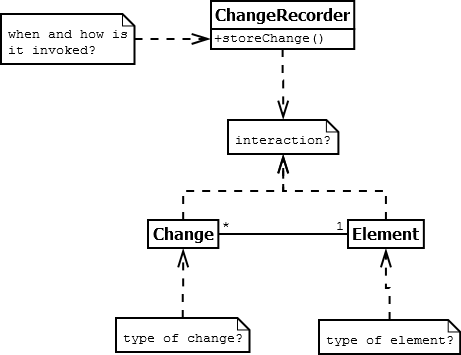
\includegraphics[width=0.8\textwidth]{Images/spec0}
\caption{Initial design speculation about recording of changes}
\label{fig:skim}
\end{figure}

\subsubsection{Initial design speculation}
With our understanding of the system, we recognized three main actors involved in this process: a change, the element that suffers the change and a change recorder that creates these two objects in some way. This can be seen in the first class diagram that we designed, shown in Figure \ref{fig:spec0}.

\subsubsection{Refined design speculation}
After examining the code for mismatches with the initial hypothesis, we adapted the class diagram in several ways, as can be seen in Figure \ref{fig:spec1}:

\begin{itemize}
\item First, we renamed the ChangeRecorder to AbstractEntityRecorder, which is at the top of the hierarchy of all change recorder classes. We also added some of the subclasses of this hierarchy like PackageRecorder, MethodRecorder and ClassRecorder. The way this AbstractEntityRecorder is invoked and by which class is still pending.

\item The Element class was renamed to Subject, which is also located at the top of the hierarchy of the elements that suffer the changes, followed by FamixObject and then all the elements like for example FamixClass, FamixPackage and FamixMethod. This was also partially extended in the diagram.

\item The Change class was also extended to show the hierarchy of change classes, by adding the subclasses specific types of changes Add, Remove and Modify.

\item Finally, the interaction between these three classes was specified, this consists in the ChangeRecorder (AbstractEntityRecorder) creating and also linking together the Change and Subject objects. The storeChange method was confirmed in the source code and is where the creation and linking takes place.
\end{itemize}

\begin{figure}[h]
\centering
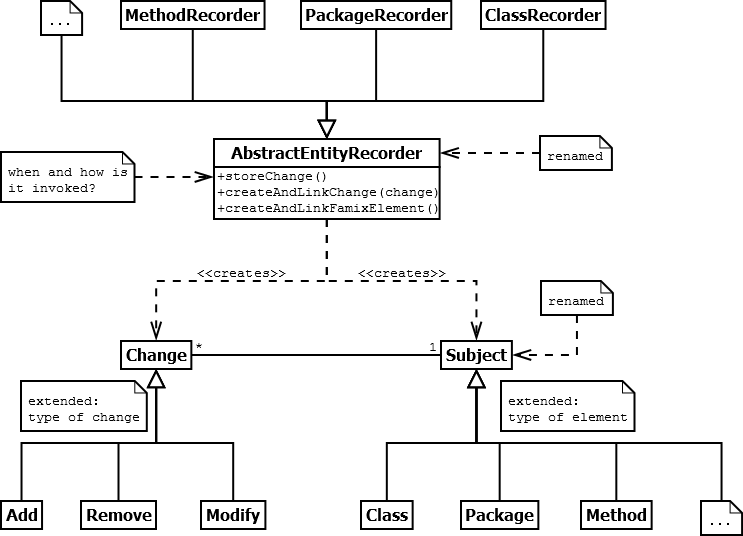
\includegraphics[width=0.8\textwidth]{Images/spec1}
\caption{Second class diagram about recording of changes}
\label{fig:spec1}
\end{figure}

\subsubsection{Final refined design}
After one last examination of the code we could answer the question remaining of how the AbstractEntityRecorder where instantiated. We found out that this is done by two classes: the ChangeRecorder class in the Logger package and the ChangeExtractor class in the Distiller package. This can be seen in Figure \ref{fig:spec2b}. This makes sense because these two packages take care of the two functionalities that store changes.

\begin{figure}[h]
\centering
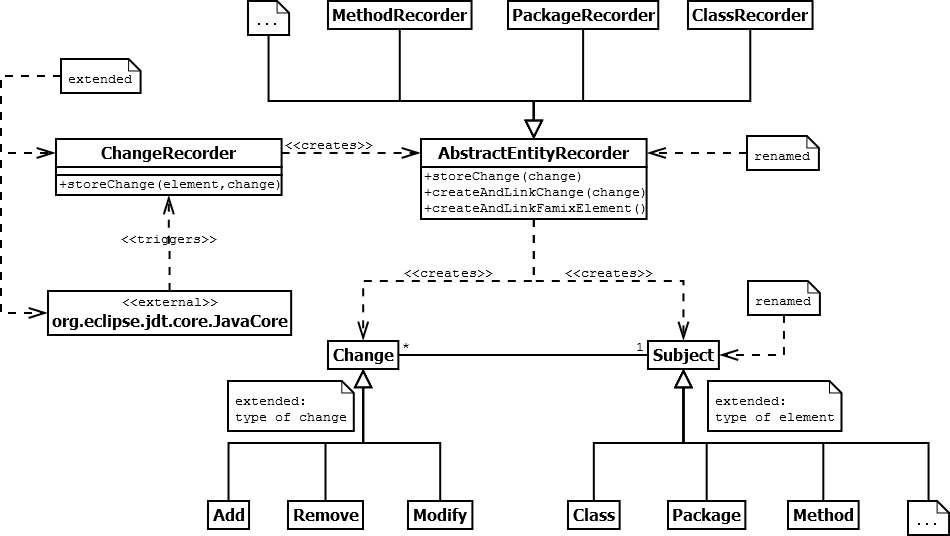
\includegraphics[width=0.9\textwidth]{Images/spec2}
\caption{Third and final class diagram about recording of changes}
\label{fig:spec2b}
\end{figure}

\subsection{Study the Exceptional Entities}
We applied this pattern to identify potential design problems related to the feature we want to reengineer. For this task we used inFusion metrics tool which we first tried in one of the lab sessions. We found this tool very useful because of the many graphical and intuitive ways it presents the results of the analyses it performs. In this section we will present and interpret three different measurements that will hopefully give us a good idea of the potential design problems in the project. 

The \emph{Overview Pyramid} provides a more general overview of relevant metrics of the project (e.g. lines of code, number of methods, number of classes), the \emph{Class Size Overview} provides a graphical representation of the sizes of the different classes in the project and the \emph{Class Inheritance} measurement provides, also graphically, an overview of all the hierarchies found in the project.

% QDI and Design Flaws
\subsubsection{QDI and Design Flaws}
First, a small note on two extra measurements that inFusion provides. For general grading of the system, inFusion employs a Quality Deficit Index (QDI), which for the initial \emph{ChEOPSJ} project is 14.1. In the documentation for the tool it is explained that the bigger the QDI is, the more significant the design problems are that the tool found. It is also worth mentioning the Number of Design Flaws, which are 26 for the initial project. Among them, two God Classes: the ModelManager class from the \emph{be.ac.ua.ansymo.cheopsj.model} package and the ClassRecorder class from the \emph{be.ac.ua.ansymo.cheopsj.changerecorders} package. Both of them are relevant to the feature we want to reengineer and are certainly exceptional entities so further analysis will be required.

%NDD = Average number of direct descendants 
%HIT = Average height of the inheritance tree
%NOP = Number of Packages
%NOC = Number of Classes
%NOM = Number of Methods
%LOC = Number of Lines of Code
%CYCLO = Sum of McCabe’s Cyclomatic Complexity for all methods
%CALL = Number of Operation Calls 
%FOUT = FANOUT = Number of Called Classes
\subsubsection{Overview Pyramid}
The Overview Pyramid for the \emph{ChEOPSJ} project can be seen in Figure \ref{fig:pyramid}.
A red color on a metric means a potential negative quantity, blue not negative or positive and green means a potential positive one.

\begin{figure}[h]
\centering
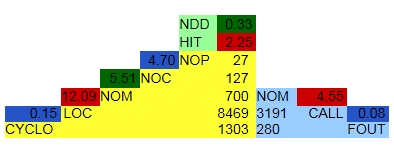
\includegraphics[width=0.7\textwidth]{Images/overviewPyramid}
\caption{Overview Pyramid for the \emph{ChEOPSJ} project by the inFusion tool}
\label{fig:pyramid}
\end{figure}

From the pyramid overview the following information can be intepreted:
\begin{itemize}
\item Class hierarchies are very tall, as it can be seen in the average height of inheritance trees (HIT) metric which is colored red with a value of 2.25. The class hierarchies are also of average width, which is good, because the average number of direct descendants (NDD) is 0.33. This observation can be seen with more detail with the Class Inheritance visualization in section \ref{sec:classInheritance}.

\item Classes have an average number of methods (5.51) and are organized in rather fine-grained packages, in other words there are few classes per package. We noticed the latter while Reading The Code In One Hour in section \ref{sec:codeOneHour} which made the initial understanding of the system easier because of the good division of classes in the packages.

\item Methods are rather long (12 lines of code per method in average), but on the other hand their logic is simple because there are not many conditional branches in the methods. This is calculated by dividing the total lines of code (LOC) by the cyclomatic complexity (CYCLO). Methods also have high coupling intensity which means that they call many methods, the number of methods (NOM) divided by the operation calls (CALL) is high.
\end{itemize}

\subsubsection{Class Size Overview}
To get an impression of the size and complexity of the classes constituting \emph{ChEOPSJ}, we used the Package Map view of the inFusion tool. This view presents all the classes grouped in their respective packages. Each class is represented by a rectangle where the width is the amount of attributes and the height the amount of methods it contains. This Package Map can be seen in Figure \ref{fig:sizeOverview}. Three potential exceptional entities are labeled in it which we will discuss further in this section.

\begin{figure}[h]
\centering
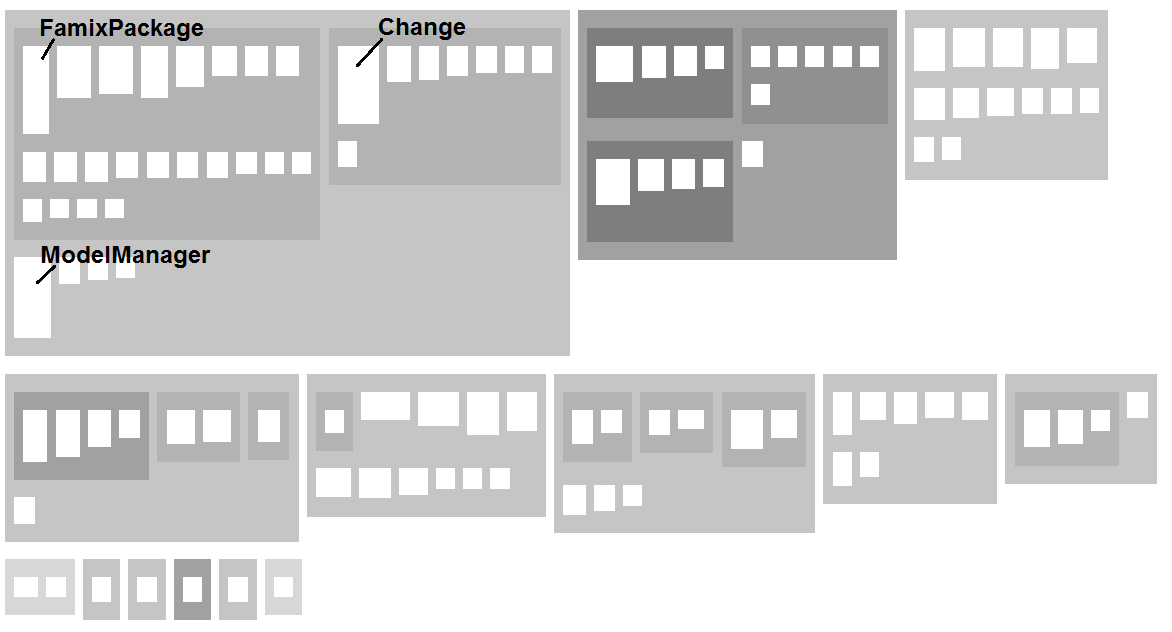
\includegraphics[width=1\textwidth]{Images/classSizeOverview}
\caption{Class size overview}
\label{fig:sizeOverview}
\end{figure}

The FamixPackage class is taller than the other classes in it's package, which means that it contains more methods. Upon closer examination in the source code we saw that these extra methods for managing the entities contained in it. This makes sense because the package is the highest level entity in a workspace and can contain all the others entities (e.g. classes, variables).

The Change class also stands out from the other classes in that it is tall and wide compared to the rest. After examining the source code we saw that all the methods are actually getters and setters and that this class does not contain much actual behavior. It is used more for storing properties of a change, like its time stamp, its intent and its dependencies -- therefore its larger width.

The ModelManager class is perhaps the most exceptional class, in its size showed in the Package Map as well as in its source code. The model manager keeps track of all the famix entities in HashMap data structures as well of the changes that these suffer, so it contains many attributes as well as getter and setter methods for those attributes. 

This class is also labeled as a God Class by the inFusion tool. It is reported by the tool that it uses many attributes from external classes, is excessively large and complex and is very non-cohesive. After examining the code and with the help of the tool, we saw that the three issues are mainly caused by a single method called printGraphForGroove. At first sight, it would appear that this method is only related to the graphical interface but further examination could be required to see if actual splitting of the god class is required.

\subsubsection{Class Inheritance}
\label{sec:classInheritance}
Next, we studied the various subtrees in the inheritance hierarchies. For visualizing them, we used the Inheritance Map from the inFusion tool which can be seen in Figure \ref{fig:inheritanceMap}. We examine three inheritance subtrees that are related to the improvement that we want to re-engineer: 

\begin{itemize}
\item The first is the one rooted at \emph{Subject}, which contains all the possible entities of a Java workspace that can suffer a change -- like Package, Class or Method. This is the deepest hierarchy with 4 levels of inheritance. The first level of inheritance seems a little suspicious because it only contains one class with no siblings which could mean that the super and subclass are not very different. This could be re-factored by merging the two classes together. This should be first verified via code browsing.

\item Next, there is the \emph{Change} hierarchy, which is quite small and straightforward. This hierarchy does not seem suspicious so we will not re-factor it following the \textbf{If It Ain’t Broke, Don’t Fix It} pattern.

\item The hierarchy of the change recorders with \emph{AbstractEntityRecorder} as the root contains a change recorder class almost for each entity of the Subject hierarchy. If we recall from previous sections, the change recorders are responsible for creating the changes and entities as well as linking them together whenever an event is sent from the eclipse framework itself saying that the user modified the compilation unit. This hierarchy seems a bit broad at the first depth level and could perhaps also use refactoring to make it more efficient and easier to extend. The root class is very small, it is actually smaller than all it's subclasses which could be solved by pushing some common methods and attributes upwards.
\end{itemize}

\begin{figure}[h]
\centering
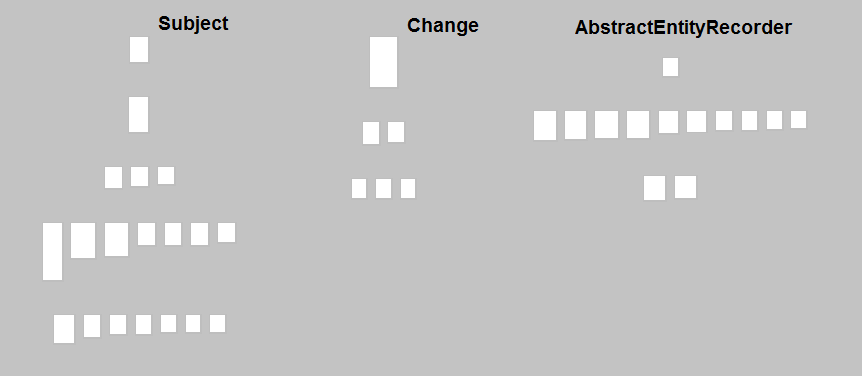
\includegraphics[width=0.8\textwidth]{Images/inheritanceMap}
\caption{Inheritance Map created with inFusion}
\label{fig:inheritanceMap}
\end{figure}

\subsubsection{God classes}
% God class ModelManager
Furthermore, as we suspected inFusion discovered the class ModelManager from the package cheopsj.model as a God class. This class is one of the largest and most complex classes in the whole system. Its job is to store and maintain every famix element created and also take care of all the changes created by the change recorders, that is the reason why this class is very complex and its coupling with the rest of the system is very high. On Figure \ref{fig:godClassMM} the graphical representation of the whole model package can be seen, where the ModelManager class is located in the left-bottom corner, colored with strong red color. Judging by the hight, width and color of the class (which represent the number of methods, attributes and design flaws respectfully) it can be concluded that the class ModelManager is a God Class indeed.

\begin{figure}[h]
\centering
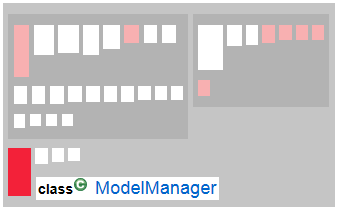
\includegraphics[width=0.5\textwidth]{Images/GodClassMM}
\caption{Graphical representation of the package cheopsj.model with inFusion}
\label{fig:godClassMM}
\end{figure}

InFusion has brought up some facts about the god class and suggested some actions that could be taken. The first fact was that ModelManager uses a lot of attributes from external classes which was very obvious from the first look at the code, because those attributes are necessary for correct functioning of the numerous methods used for managing of the processes in the model. The second fact was that this class is excessively large and complex and the reason for that are the methods, which have high cyclomatic complexity (a lot of branching in the code) and high nesting level. The biggest and most complex method is printGraphForGroove(), which has a heavy code branching and deep nesting. Also this method has very weak encapsulation because it calls a lot of external accessors.

% God class ClassRecorder
The second most complex and also God Class is ClassRecorder, which is located in the changerecorders package and its job is to record every change done to the famixClass element. This class has very weak cohesion with the system because its methods are rarely called and on the other hand it calls a large number of external methods. ClassRecorder is also non-cohesive because its methods does not use its attributes very often, for example the method findParentName is using none of the attributes of the class.

The usage of inFusion has helped us a lot for better understanding of the complexity of the system and detection of some of the design flaws. What really makes the job easier is the graphical representation of some of the most important features of an object-oriented code in our case Java, like encapsulation, cohesion, size, complexity, hierarchies. The small drawback of this method is that there are so many statistics and they are increasing with every other tool, that the developer can sometimes get carried away in a direction away from the essential problems of the design. Also the tools like inCode or inFusion only represent the information collected from the source code, but none of them offers some kind of a solution to some of the design flaws encountered.

\section{Detailed Model Capture}
\subsection{Refactor to Understand}
This chapter presents some of the refactoring we have done to the plugin, which also helped us to better understand the system. Three types of refactoring techniques we have used and they will be explained in the following paragraphs.

\subsubsection{Remove Duplicate Code}
For locating the duplicated code we have used the tool CCFinderX which was used on the duplicated code laboratory session. One of the biggest and most important duplicate code we have refactored is the method \emph{setStructuralDependencies} that was located in two classes: ClassRecorder and MethodRecorder in the package \emph{be.ac.ua.ansymo.cheopsj.changerecorders}. This method was used by both of the mentioned classes in order to manage the structural dependencies between the changes, depending on if the change was of type addition or removal of classes or methods.
After the duplicated code was located and we have seen that both of the classes Method and Class Recorder are part of a hierarchy where the abstract class AbstractEntityRecorder is their parent, we figured out that we can use the refactoring method \textbf{Pull Up Method}.

\begin{figure}[h]
\centering
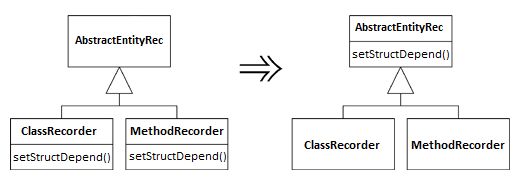
\includegraphics[width=0.9\textwidth]{Images/PullUpMethod}
\caption{Graphical representation of the Pull Up Method refactoring}
\label{fig:PullUp}
\end{figure}

The result of the refactoring is graphically represented on Figure \ref{fig:PullUp}, the method was pulled up to the common parent of the both classes and that is the AbstractEntityRecorder class. Because the setStructuralDependencies method was private it could be only used by the classes where it was declared, now after transferring it one level up in the hierarchy and making the method protected it can be used only by the methods which extend the class where it is located.

\subsubsection{Replace Condition Branches by Methods}
This refactoring method suggests that, if we locate branches in methods that have a large number of lines of code and a lot of responsibilities, they can be used to create new private methods. As an example of this kind of refactoring we are going to present how we have divided a branch of code from the method \textbf{setStructuralDependencies} which was duplicated and was refactored. This kind of refactoring is easy and the most important elements are: to locate how many and what kind of attributes the new method should receive and what it does need to return. In our case a big \emph{if} branch is replaced with private method named setStructDepAdd, which is setting the structural dependencies if the change that was made was of type \emph{Add}.

\subsubsection{Refactor Method Bodies to a Consistent Level of Abstraction}
Because long methods are a bad design solution and they can cause problems and lower the efficiency of the system, they should be refactored by removing big blocks of code and transferring them to a new private methods. This refactoring is very similar to the previous one, with the main difference instead of creating a new method from a branch, we can create new method if we find a block of code which logically represents a feature of the method. An example is the method \textbf{loadModel} in the class ModelManager, which is used for loading the model from already stored file. The block of code that loads the famix entities has been extracted from loadModel to a new private method called \textbf{loadFamixEntities} and the new method as input receives the ObjectInputStream from the file where the entities are stored.

\section{Reengineering}

\subsection{Redistribute Responsibilities}

\subsubsection{Split Up God Class}
This refactoring method is used to split the god class into a number of smaller classes which will redistribute the responsibilities from the god class. Solving this problem was difficult because the methods from the god class in our system (\textbf{ModelManager}) were receiving a big number of external calls from classes located all over the system.

From ModelManager we have extracted four classes as it can be seen on Figure \ref{fig:GodClassSplit} and in the following paragraphs we are going to explain the process of refactoring. The two most obvious fields that we could split from the ModelManager are \emph{changes} and \emph{listeners}, which are used for storing all the changes and listeners present in the system.

\begin{figure}[h]
\centering
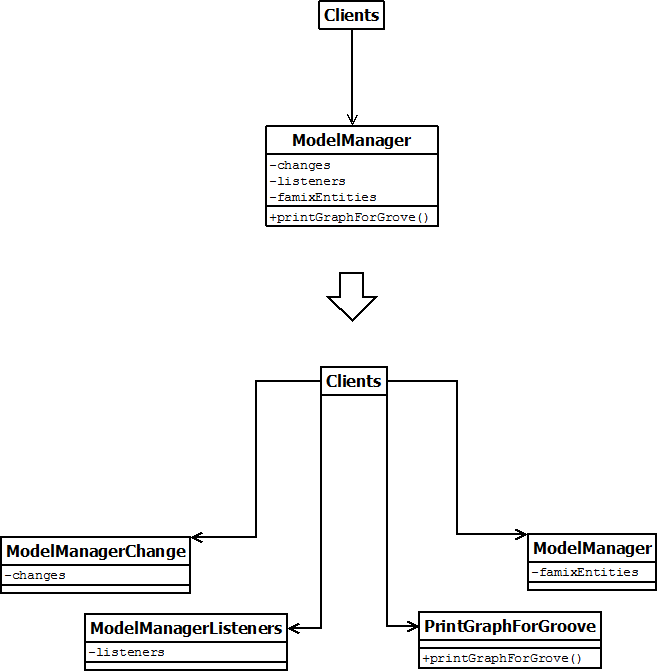
\includegraphics[width=0.9\textwidth]{Images/GodClassSplit}
\caption{Graphical representation of the Split God Class refactoring, before and after applying}
\label{fig:GodClassSplit}
\end{figure}

We have created two new classes \textbf{ModelManagerChange} and \textbf{ModelManagerListeners} that are containing the above mentioned fields and we have transferred all the methods that are managing those fields to the new classes. After we finished with the transfer of the actual code of the relevant methods, still all the external calls were coming to the ModelManager, which was then redirecting them to the new classes. To solve that problem we have located all the incoming calls to the transferred methods and we have redirected them to the new classes. Because the ModelManager is a Singleton class, which means that only one instance can exist in the whole system, we have also made the new classes Singletons.

Furthermore, we have noticed a big method called \emph{printGraphForGroove} followed with a numerous private methods used by it. This method had a lot of external outgoing calls to other methods and that is why we figured out that is a good idea to create a completely new class called \textbf{PrintGraphForGroove}. In this class we have transfered also all the private methods that were used by the printGraphForGroove method.

Lastly the class ModelManager is not deleted, but now it is not a god class. This class is now in charge of managing the entities like famix classes, methods, variables and also for loading and saving the method. All the external incoming calls are not coming to ModelManager as before the refactoring, but all of them are redirected to the class that contains the method they want to call.

After splitting the god class we have run InFusion to analyze the project and we have received some satisfying results. First of all the overall quality deficit index (QDI) was lowered from 11.9 to 7.1, which means that the refactorings we have made are correct and are providing results. As second the class ModelManager was not more recognized as a god class, but as a regular class. It is worth mentioning that the tests we have written about the ModelManager are now testing some methods from the new classes and they are not showing any failures.

\newpage
\section{References}
\begin{thebibliography}{9}

\bibitem{demeyer02}
	Demeyer, Serge, St{\'e}phane Ducasse, and Oscar Nierstrasz,
	\emph{Object-oriented reengineering patterns}. 
	Morgan Kaufmann, 
	2002.

\end{thebibliography}
\end{document}
